\chapter{Generalized Linear Models {\color{red} DRAFT} \label{chapter:glms}}

Generalized linear models (GLMs) are a class of supervised learning models that form a convenient bridge between machine learning and traditional statistics. The basic idea behind a GLM is that your outcome variable (a.k.a. response variable, see Chapter~\ref{chapter:classification}), $y$, follows a probability distribution. A linear function of the predictors (a.k.a. covariates, again see Chapter~\ref{chapter:classification}), $x_1, \dots, x_p$, explains where the mean of that distribution is, but there is still some random spread around that mean due to factors that aren't modeled, plus noise.

Today, we will focus on three classes of GLM: \textbf{linear regression}, which models data where the outcome, $y$, is numeric $\left( y \in \mathbb{R} \right)$; \textbf{logistic regression}, in which the outcome is binary $\left( y \in \{0, 1\} \right)$, and \textbf{loglinear (Poisson) regression}, in which the outcome is a positive integer, or count $\left( y \in \{0, 1, 2, \dots\} \right)$. \\

%%%%%%%%%%%%%%%%%%%%%%%%%%%%%%%%%%%%%%%%%%%%%%%%%%%%%%%%%%%%%%%%%%%%%%%%%%%%%%%

\section{Model Assumptions}

In GLMs, the predictors can be anything -- interval, ordinal, or nominal -- regardless of the specific model one chooses. However, there are several other assumptions that are important to consider before fitting one of these models:

\begin{itemize}
\item We assume that the outcome follows a certain type of distribution (e.g. Bernoulli distribution for a logistic regression model, normal for linear, etc.). That assumption is baked into the model structure. It is, therefore, important to consider whether the outcome distribution you chose actually makes sense for your particular problem.
\item We assume that the predictors are fixed and known, and thus have no error associated with their measurements (Bayesian versions of these models relax this assumption).
\item We assume that the predictors enter the model as a linear combination (this is what makes these ``linear models''). 
\item We assume that the $n$ samples in our dataset are collected independently, so that the errors of the $n$ responses are uncorrelated. (Another way of thinking about this is that the outcomes are drawn iid from the relevant distribution.)
\item We assume that the predictors are not collinear. If they are, it can lead to model instability even if the model appears to predict the outcome well. 
\end{itemize}

%%%%%%%%%%%%%%%%%%%%%%%%%%%%%%%%%%%%%%%%%%%%%%%%%%%%%%%%%%%%%%%%%%%%%%%%%%%%%%%

\section{Modeling the Outcome}

\subsection{Linear Regression}

The linear regression model has a long history of development before the advent of GLMs, so it's typically taught in its own course with all of the associated model diagnostics, goodness of fit tests, etc. long before a student ever sees other GLMs. I think a comparative approach is more effective, which is why we're doing it this way.

\paragraph{Outcome Distribution: Normal} In linear regression, we assume that the outcome, $y$, is normal. Recall that the normal distribution is a continuous probability distribution with the following properties:
$$ p(y | \mu, \sigma) = \frac{1}{\sqrt{2 \pi \sigma^2}} e^{-\frac{(y-\mu)^2}{2 \sigma^2}} \qquad  E[y| \mu, \sigma] = \mu \qquad \text{var}(y | \mu, \sigma) = \sigma^2 $$
where $y \in \mathbb{R}$.

\subsection{Logistic Regression}

Logistic regression models data where the outcome is binary; i.e. where $y$ is ``yes'' or ``no''. Variants of logistic regression, called \textbf{multinomial logistic regression} and the \textbf{proportional odds model}, can also be used to model data where the outcome contains multiple categories that either have an ordering (ordinal) or do not (nominal). We will see how this works in a second.

\paragraph{Outcome Distribution: Bernoulli} In logistic regression, we assume that the outcome, $y$, is either $0$ or $1$. We model it using the Bernoulli distribution, which is a discrete probability distribution with the following properties:
$$ p(y|\mu) = \mu^y (1 - \mu) ^ {1-y} \qquad E[y| \mu] = \mu \qquad \text{var}(y | \mu) = \mu (1 - \mu) $$
where $y \in \{0, 1\}$.

\subsection{Loglinear (Poisson) Regression}

In Poisson regression, the outcome is a count. This type of regression is less common than linear and logistic regression, but we include it here mainly so you can see how the ideas from GLM extend to many different classes of outcome distributions within the exponential family. 

\paragraph{Outcome Distribution: Poisson} In Poisson regression, we model the outcome using the Poisson distribution, which is a discrete probability distribution with the following properties:
$$ p(y | \lambda) = \frac{e^{-\lambda} \lambda^y}{y!} \qquad E[y|\lambda] = \lambda \qquad \text{var}(y|\lambda) = \lambda $$
where $y \in 0, 1, 2, \dots$.

%%%%%%%%%%%%%%%%%%%%%%%%%%%%%%%%%%%%%%%%%%%%%%%%%%%%%%%%%%%%%%%%%%%%%%%%%%%%%%%

\section{Modeling the Predictors}

All of the models we will see today incorporate a \textbf{linear combination} of predictors. A linear combination is an expression constructed from a set of terms by multiplying each term by a constant and adding the results.

We denote the number of predictors in the model by $p$, and denote the vector of predictors by $x$, where
$$ x = \begin{bmatrix}
1 \\
           x_{1} \\
           x_{2} \\
           \vdots \\
           x_{p}
         \end{bmatrix} $$
and we have included a ``1'' as the first element to allow for an \textbf{intercept}. We write $x^{(i)}$ to denote the vector of predictors associated with the $i$th training example.

The coefficients of the linear combination (i.e. the model parameters we are hoping to learn) are denoted by:
$$ \beta = \begin{bmatrix}
\beta_0 \\
           \beta_{1} \\
           \beta_{2} \\
           \vdots \\
           \beta_{p}
         \end{bmatrix} $$
and we often express the linear combination as an inner product, written as:
$$ \beta^T x = \beta_0 + \sum_{j=1}^p \beta_j x_j. $$

%%%%%%%%%%%%%%%%%%%%%%%%%%%%%%%%%%%%%%%%%%%%%%%%%%%%%%%%%%%%%%%%%%%%%%%%%%%%%%%

\section{Linking the Predictors to the Outcome}

All of the models we see today model the \textbf{expected value} of the outcome, $E[y]$ as some function of this linear combination of predictors. The function that relates the two is called the \textbf{link function}. Different types of regression use different link functions.

\subsection{Linear Regression} 

In linear regression, the mean of the outcome distribution, which is normal, can be any real number. We therefore use the \textbf{identity link}, setting $E[y]$ directly equal to the linear combination of predictors. Since the outcome is normal, we know that $E[y] = \mu$, the mean of the normal distribution. We therefore write:
\begin{equation} E[y] = \mu = \beta^T x \label{eqn:meanlinear} \end{equation}
which is usually rearranged and rewritten as:
$$ y = \beta^T x + \varepsilon $$
where $\varepsilon \sim N(0, \sigma^2)$. The relationship between $E[y]$ and $\beta^T x$ is shown below.

\begin{center}
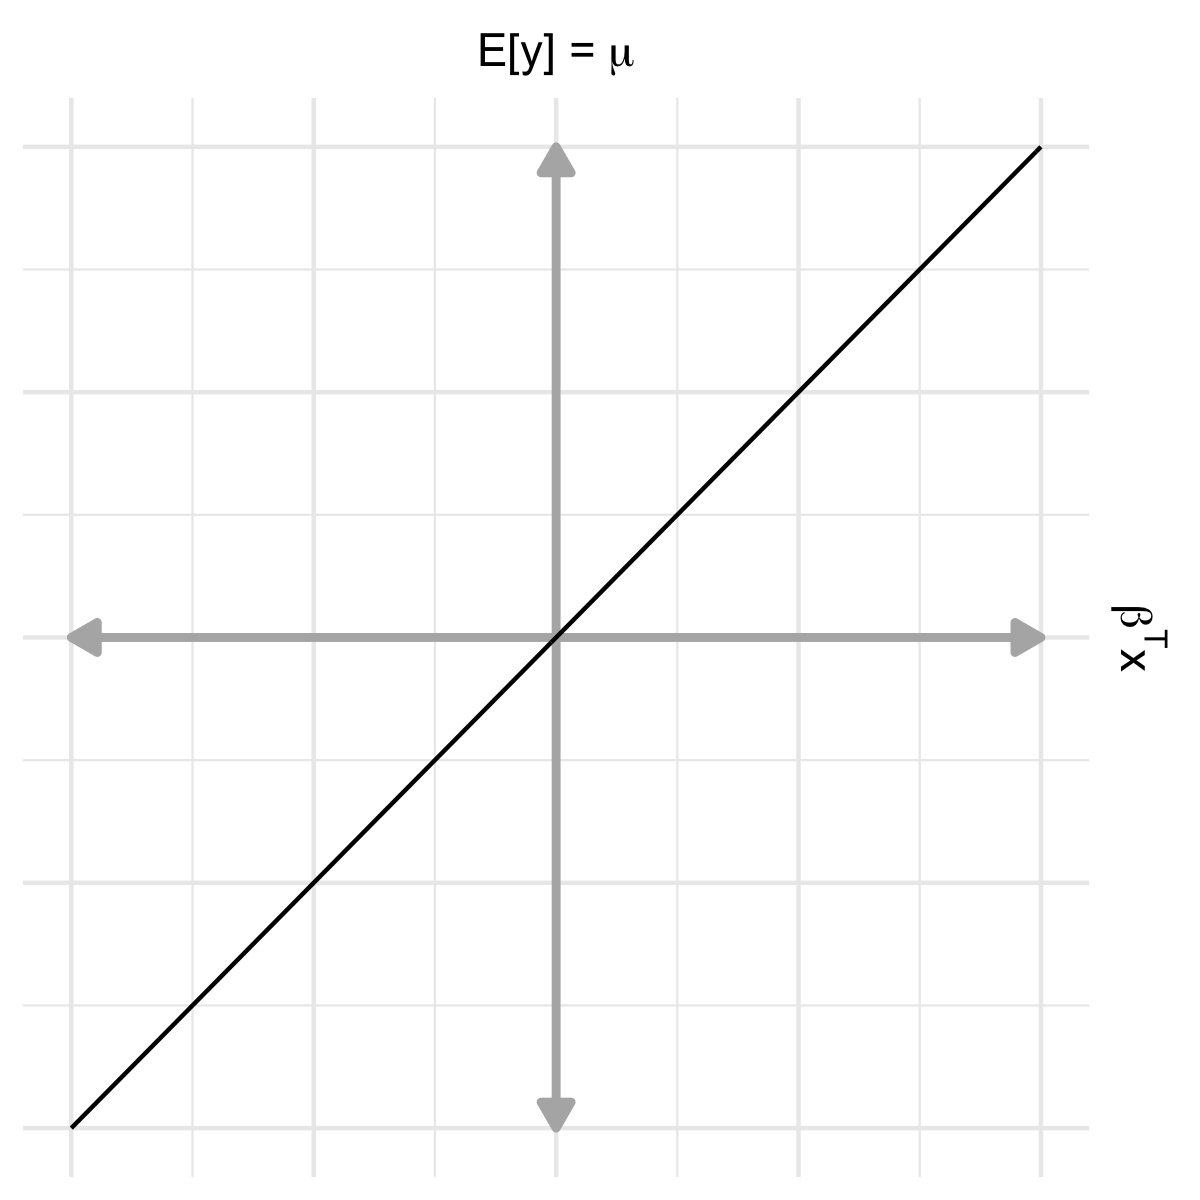
\includegraphics[width=0.6\textwidth]{img/l02-figure1-linreg.png}
\end{center}

\subsection{Logistic Regression}

In logistic regression, the mean of the outcome distribution, which is Bernoulli, is a probability. It must therefore be a real number between 0 and 1. No matter how large or small $\beta^T x$ gets, the value of $E[y] = \mu$ cannot be outside this range. We therefore apply the \textbf{logistic function}, $f(x) = 1/(1 + \exp(-x))$, which has the range $(0, 1)$, to $\beta^T x$ to squash it:
\begin{equation} E[y] = \mu = \frac{1}{1 + \exp{(-\beta^Tx)}} \label{eqn:meanlogistic} \end{equation}
The relationship between $E[y]$ and $\beta^T x$ is shown below. We typically invert the model to write
$$ \log{\frac{\mu}{1-\mu}} = \beta^T x $$
which is the standard form of the logistic regression model. The function $\log \left( \mu/(1-\mu) \right)$ is called the logit, and in logistic regression we say we use the \textbf{logit link}.

\begin{center}
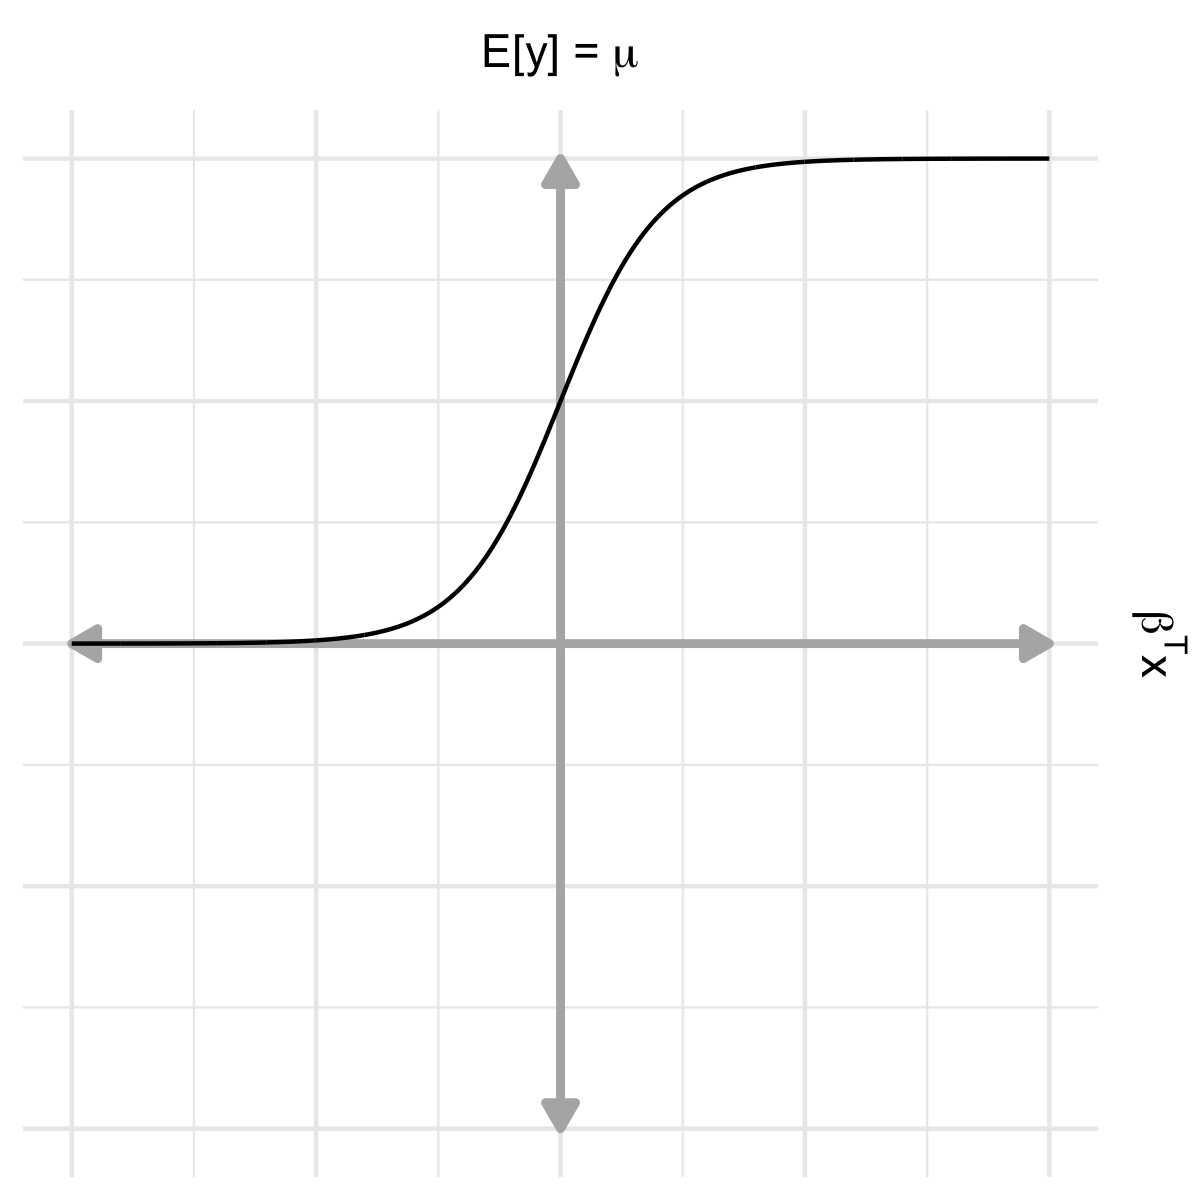
\includegraphics[width=0.6\textwidth]{img/l02-figure2-logistic.png}
\end{center}

\subsection{Loglinear (Poisson) Regression}

In Poisson regression, the mean of the outcome distribution, which is Poisson, is the expected value of a count. It must therefore be a real number greater than or equal to zero. In particular, no matter how small $\beta^T x$ gets, the value of $E[y] = \lambda$ cannot be negative. We therefore exponentiate $\beta^T x$ to ensure that the result is greater than zero:
\begin{equation} E[y] = \lambda = \exp(\beta^T x) \label{eqn:meanpoisson} \end{equation}
The relationship between $E[y]$ and $\beta^T x$ is shown below. We typically invert the model to write
$$ \log(\lambda) = \beta^T x $$
which is the standard form of the Poisson regression model. We say we use the \textbf{log link}. 

\begin{center}
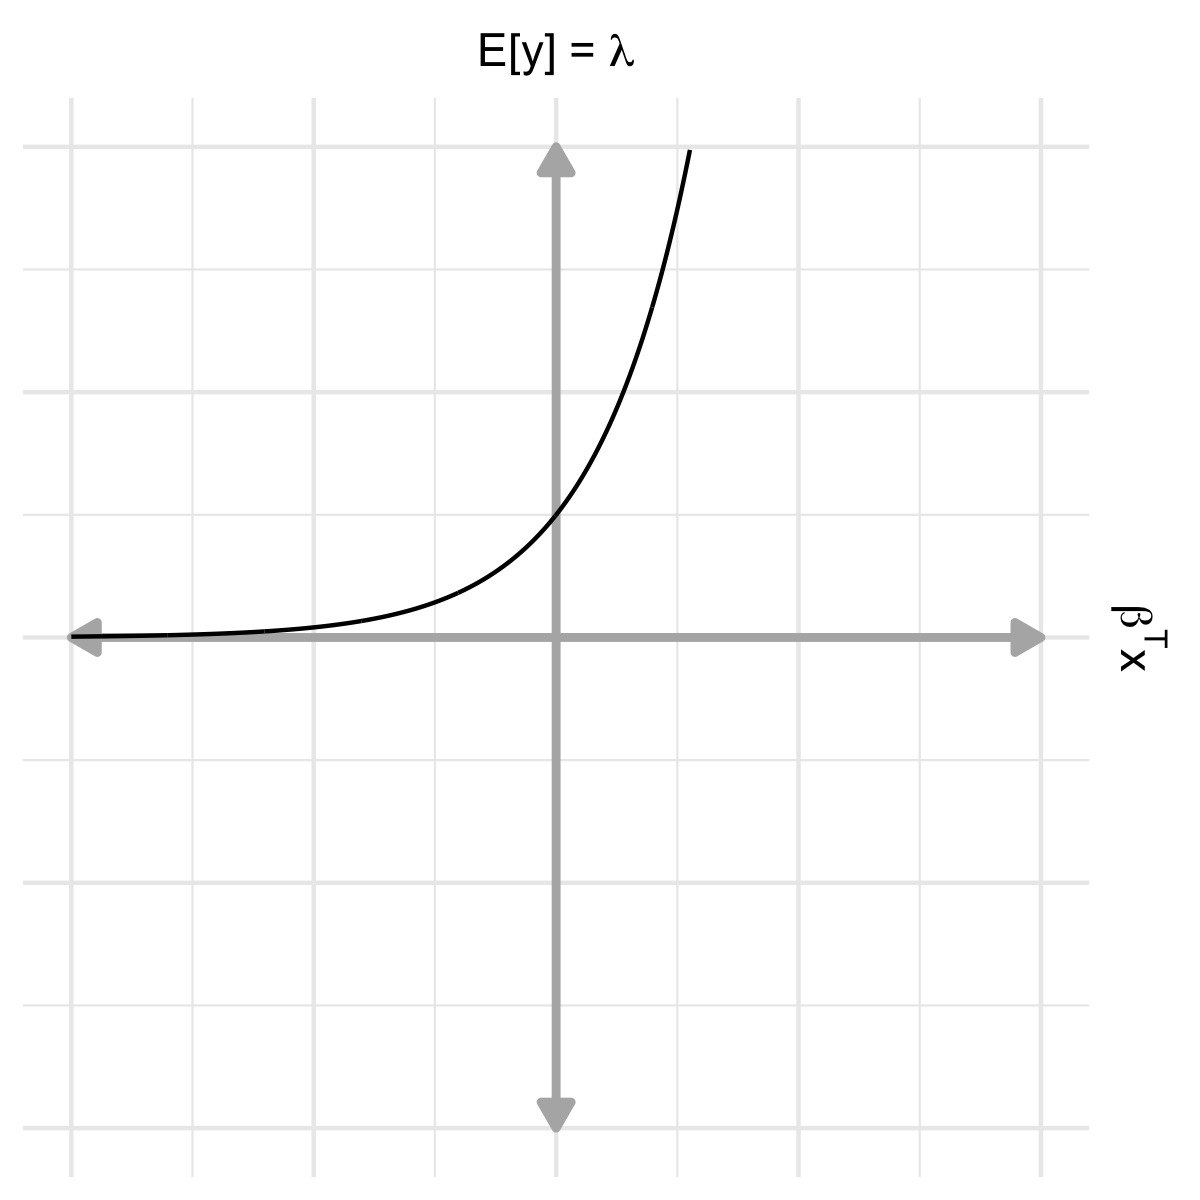
\includegraphics[width=0.6\textwidth]{img/l02-figure3-poisson.png}
\end{center}

%%%%%%%%%%%%%%%%%%%%%%%%%%%%%%%%%%%%%%%%%%%%%%%%%%%%%%%%%%%%%%%%%%%%%%%%%%%%%%%

\section{Fitting GLMs}

GLMs are typically fit using maximum likelihood estimation (see Chapter~\ref{chapter:mlebasics}). A full treatment of MLE for GLMs is outside the scope of these notes, but I've put the start of the calculations for each type of model below.    

\subsection{Linear Regression} 

The likelihood for the linear regression model is:
$$ \mathcal{L}(\mu^{(1)}, \dots, \mu^{(n)}, \sigma) = \prod_{i=1}^n \frac{1}{\sqrt{2 \pi \sigma^2}} \exp \left[ - \frac{(y^{(i)} - \mu^{(i)})^2}{2 \sigma^2} \right] $$
where we use $\mu^{(i)}$ to represent the model's estimate of the mean of the outcome at the position of training example $i$. We can use Equation~\ref{eqn:meanlinear} to rewrite this as a function of the predictors:
$$ \mathcal{L}(\beta, \sigma) = \prod_{i=1}^n \frac{1}{\sqrt{2 \pi \sigma^2}} \exp \left[ - \frac{(y^{(i)} - \beta^T x^{(i)})^2}{2 \sigma^2} \right] $$
Taking the log, we obtain the log-likelihood:
$$ \log \mathcal{L}(\beta, \sigma) = -\frac{n}{2} \log (2 \pi) - \frac{n}{2} \log(\sigma^2) - \frac{1}{2 \sigma^2} \sum_{i=1}^n \left( y^{(i)} - \beta^T x^{(i)} \right)^2 $$
Taking derivatives of the log-likelihood with respect to the $\beta$s, we find that we can maximize the likelihood by minimizing the sum-squares: $\sum_{i=1}^n \left( y^{(i)} - \beta^T x^{(i)} \right)^2$.

\subsection{Logistic Regression}

The likelihood for the logistic regression model is:
$$ \mathcal{L}(\mu^{(1)}, \dots, \mu^{(n)}) = \prod_{i=1}^n {\mu^{(i)}}^{y^{(i)}} (1-\mu^{(i)})^{1 - y^{(i)}} $$
Rewriting this as a function of the predictors, we get:
$$ \mathcal{L}(\beta) = \prod_{i=1}^n \left( \frac{1}{1 + \exp(-\beta^T x^{(i)})} \right)^{y^{(i)}} \left( \frac{\exp(-\beta^T x^{(i)})}{1 + \exp(-\beta^T x^{(i)})} \right)^{1 - y^{(i)}} $$
Taking the log, we obtain the log-likelihood:
$$ \log \mathcal{L}(\beta) = \sum_{i=1}^n \left[ -y^{(i)} \log \left[ 1 + \exp(-\beta^T x^{(i)}) \right] + (1 -y^{(i)}) \log \left[ 1 + \exp(-\beta^T x^{(i)}) \right] \right] $$
Again, we will take derivatives of the log-likelihood with respect to the $\beta$s to maximize it. However, we cannot solve for the optimal $\beta$s analytically; numerical optimization methods are used to perform the optimization.

\subsection{Loglinear (Poisson) Regression}

The likelihood for the Poisson regression model is:
$$ \mathcal{L}(\lambda^{(1)}, \dots, \lambda^{(n)}) = \prod_{i=1}^n \frac{{\lambda^{(i)}}^{y^{(i)}} e^{-\lambda^{(i)}}}{y^{(i)}!} $$
Rewriting this as a function of the predictors, we get:
$$ \mathcal{L}(\beta) = \prod_{i=1}^n \frac{\exp{(y^{(i)} \beta^T x^{(i)})} e^{-\exp{(\beta^T x^{(i)})}}}{y^{(i)}!} $$
Taking the log, we obtain the log-likelihood:
$$ \log \mathcal{L}(\beta) = \sum_{i=1}^n \left[ y^{(i)} \beta^T x^{(i)} - \exp(\beta^T x^{(i)}) - \log (y^{(i)}!) \right] $$
As with logistic regression, we cannot solve for the optimal $\beta$s analytically; numerical optimization methods are used. 


